% !TEX root = ../../STP_IoTjournal.tex
\subsection{Setup \label{sec:city_simSetup}}
We grid the City of San Francisco (SF) in California, USA, and use it as our position space, as shown in Fig. \ref{fig:sf_setup}. 
\begin{figure}
  \centering
  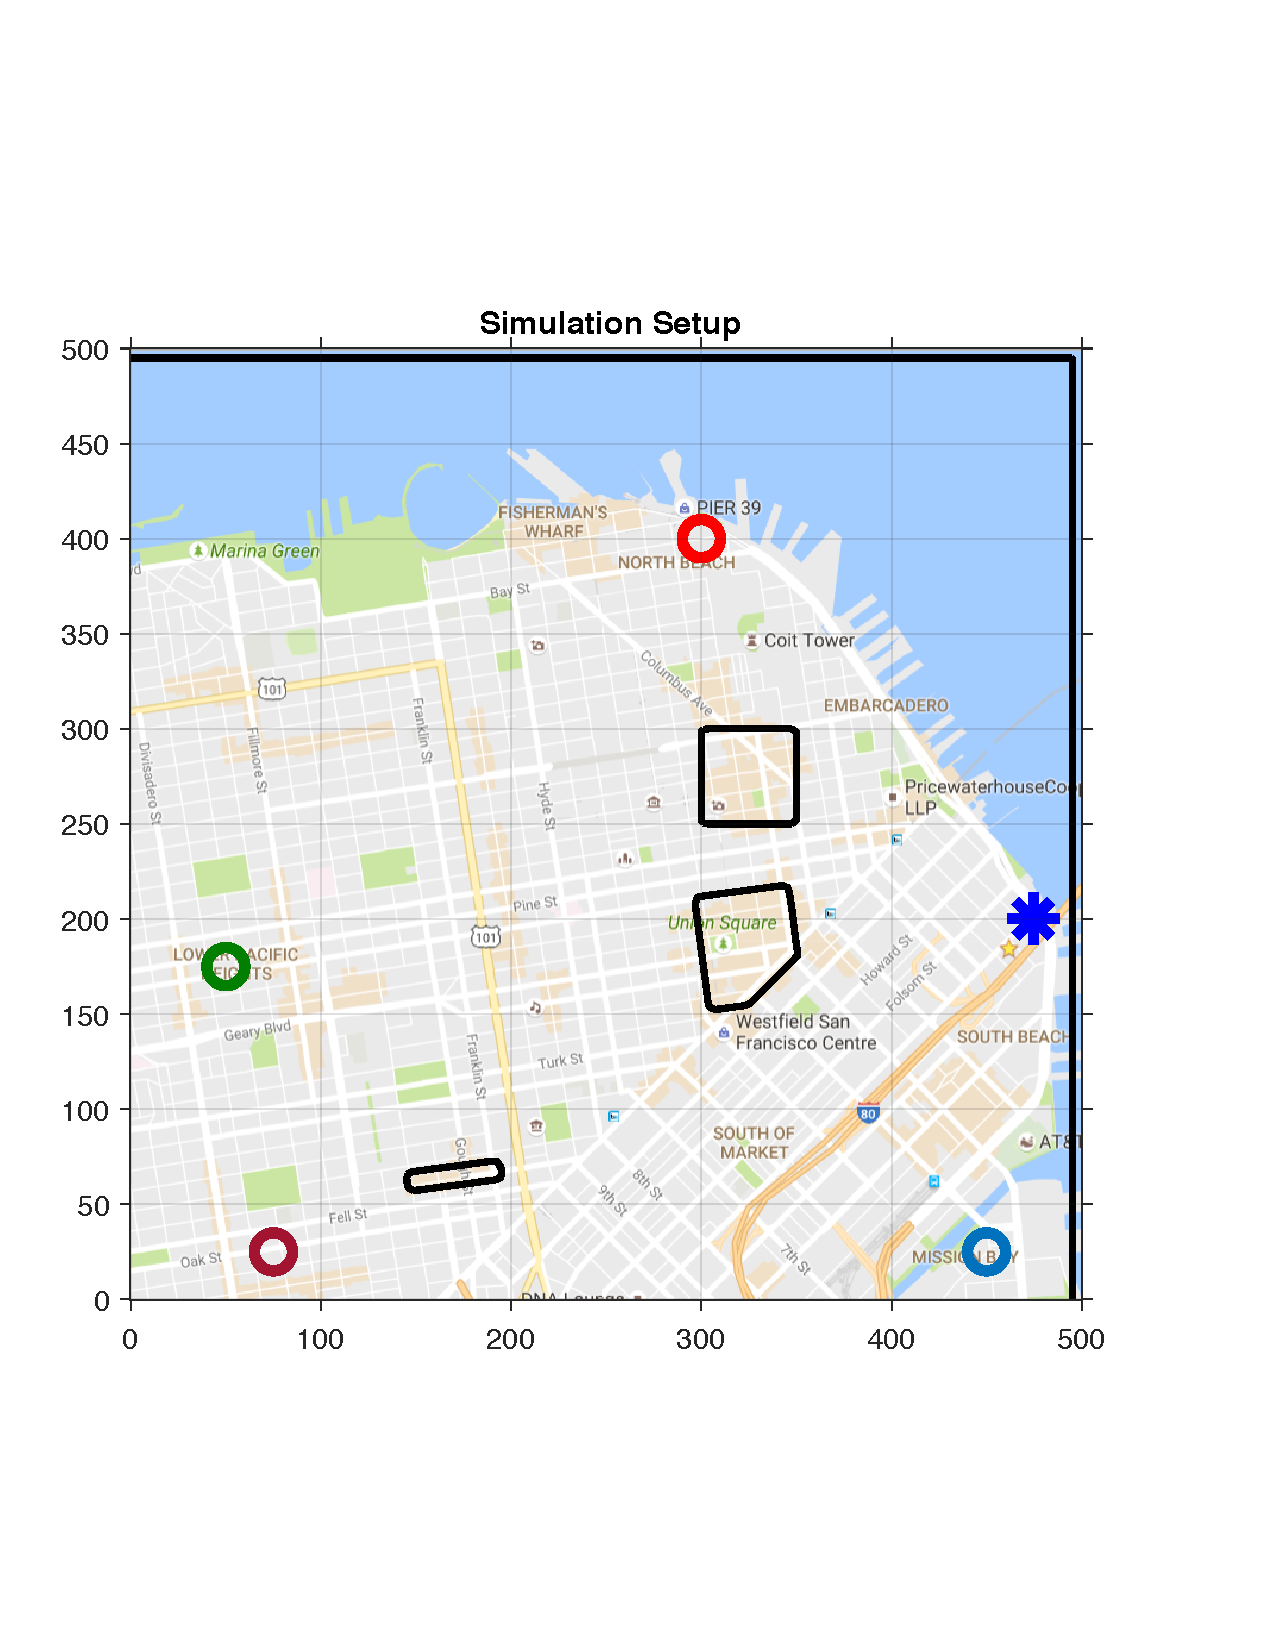
\includegraphics[width=\columnwidth]{figs/sf_setup}
  \caption{Simulation setup. A $25$ km$^2$ area in the City of San Francisco is used as the space for the STP vehicles. STP vehicles originate from the blue star and go to one of the four destinations, denoted by circles. Tall buildings in the downtown area are used as static obstacles, represented by the black contours.}
  \label{fig:sf_setup}
\end{figure}
Each box in Fig. \ref{fig:sf_setup} represents a $1$ km$^2$ area of SF. The origin point for the vehicles is denoted by the blue star. Four different areas in the city are chosen as the destinations for the vehicles. Mathematically, the target sets $\targetset_i$ of the vehicles are circles of radius $r$ in the position space, i.e. each vehicle is trying to reach some desired set of positions. In terms of the state space $\state_i$, the target sets are defined as
\begin{equation}
\label{eq:target_sim}
\targetset_i = \{\state_i: \|\pos_i - c_i\|_2 \le r\}
\end{equation}
\noindent where $c_i$ are centers of the target circles. In this simulation, we use $r = 100$ m. The four targets are represented by four circles in Fig. \ref{fig:sf_setup}. The destination of each vehicle is chosen randomly from these four destinations. Finally, some areas in downtown SF and the city hall are used as representative static obstacles for the STP vehicles, denoted by black contours in Fig. \ref{fig:sf_setup}.

For this simulation, we use the following dynamics for each vehicle:
\begin{equation}
\label{eq:dyn_i}
\begin{aligned}
\dot{\pos}_{x,i} &= v_i \cos \theta_i + \dstb_{x,i} \\
\dot{\pos}_{y,i} &= v_i \sin \theta_i + \dstb_{y,i}\\
\dot{\theta}_i &= \omega_i, \\
& \underline{v} \le v_i \le \bar{v}, ~|\omega_i| \le \bar{\omega}, \\
& \|(\dstb_{x,i}, \dstb_{y,i}) \|_2 \le d_{r}
\end{aligned}
\end{equation}
\noindent where $\state_i = (\pos_{x,i}, \pos_{y,i}, \theta_i)$ is the state of vehicle $\veh_i$, $\pos_i = (\pos_{x,i}, \pos_{y,i})$ is the position, $\theta_i$ is the heading, and $d = (d_{x,i}, d_{y,i})$ represents $\veh_i$'s disturbances, for example wind, that affect its position evolution. The control of $\veh_i$ is $u_i = (v_i, \omega_i)$, where $v_i$ is the speed of $\veh_i$ and $\omega_i$ is the turn rate; both controls have a lower and upper bound. To make our simulations as close as possible to real scenarios, we choose velocity and turn-rate bounds as $\underline{v} = 0$ m/s, $\bar{v} = 25$ m/s, $\bar\omega = 2$ rad/s, aligned with the modern UAV specifications \cite{UAVspecs1, UAVspecs2}. The disturbance bounds are chosen to be either $\dstb_r = 6$ m/s or $\dstb_r= 11$ m/s. These conditions correspond to \textit{moderate breeze} and \textit{strong breeze} respectively on the Beaufort scale \cite{Windscale}. The scheduled times of arrival $\sta_i$ for all vehicles are chosen to be all $0$ for a high UAV density condition. For medium and low density conditions, we separated the $\sta_i$ for the vehicles by $5$ s and $10$ s respectively, with the latest $\sta_i$ being 0. Note that we have used same dynamics and input bounds across all vehicles for clarity of illustration; however, STP can easily handle more general systems of the form in which the vehicles have different control bounds, $\sta_i$ and dynamics.

The goal of the vehicles is to reach their destinations while avoiding a collision with the other vehicles or the static obstacles. The joint state space of this 50-vehicle system is 150-dimensional (150D), making the joint trajectory planning and collision avoidance problem intractable for direct analysis. Therefore, we assign a priority ordering to vehicles and solve the trajectory planning problem sequentially. For this simulation, we assign a random priority order to fifty vehicles and use RTT algorithm to compute the trajectories of the vehicles. 